% Digital Logic Report Template
% Created: 2020-01-10, John Miller

%==========================================================
%=========== Document Setup  ==============================

% Formatting defined by class file
\documentclass[11pt]{article}

% ---- Document formatting ----
\usepackage[margin=1in]{geometry}	% Narrower margins
\usepackage{booktabs}				% Nice formatting of tables
\usepackage{graphicx}				% Ability to include graphics

%\setlength\parindent{0pt}	% Do not indent first line of paragraphs 
\usepackage[parfill]{parskip}		% Line space b/w paragraphs
%	parfill option prevents last line of pgrph from being fully justified

% Parskip package adds too much space around titles, fix with this
\RequirePackage{titlesec}
\titlespacing\section{0pt}{8pt plus 4pt minus 2pt}{3pt plus 2pt minus 2pt}
\titlespacing\subsection{0pt}{4pt plus 4pt minus 2pt}{-2pt plus 2pt minus 2pt}
\titlespacing\subsubsection{0pt}{2pt plus 4pt minus 2pt}{-6pt plus 2pt minus 2pt}

% ---- Hyperlinks ----
\usepackage[colorlinks=true,urlcolor=blue]{hyperref}	% For URL's. Automatically links internal references.

% ---- Code listings ----
\usepackage{listings} 					% Nice code layout and inclusion
\usepackage[usenames,dvipsnames]{xcolor}	% Colors (needs to be defined before using colors)

% Define custom colors for listings
\definecolor{listinggray}{gray}{0.98}		% Listings background color
\definecolor{rulegray}{gray}{0.7}			% Listings rule/frame color

% Style for Verilog
\lstdefinestyle{Verilog}{
	language=Verilog,					% Verilog
	backgroundcolor=\color{listinggray},	% light gray background
	rulecolor=\color{blue}, 			% blue frame lines
	frame=tb,							% lines above & below
	linewidth=\columnwidth, 			% set line width
	basicstyle=\small\ttfamily,	% basic font style that is used for the code	
	breaklines=true, 					% allow breaking across columns/pages
	tabsize=3,							% set tab size
	commentstyle=\color{gray},	% comments in italic 
	stringstyle=\upshape,				% strings are printed in normal font
	showspaces=false,					% don't underscore spaces
}

% How to use: \Verilog[listing_options]{file}
\newcommand{\Verilog}[2][]{%
	\lstinputlisting[style=Verilog,#1]{#2}
}




%======================================================
%=========== Body  ====================================
\begin{document}

\title{ELC 2137 Lab 2: Transistor Logic Gates}
\author{Jake Simmons and Haonan Jin}
\maketitle

\section*{Summary}

The purpose of this lab was to build and explore the behviors of logic gates. We first built an OR Gate, second a Not Gate and third a Nor Gate. The last logic gate was a combination of two Not Gates and a single Nor Gate.      


\section*{Q\&A}

\begin{enumerate}
	\item What logic operation does the Final gate implement?
		\begin{enumerate}
			\item The logic operation that the Final gate implements is an And Gate.
		\end{enumerate}
\end{enumerate}



\section*{Results}
\begin{center}
\begin{figure}
		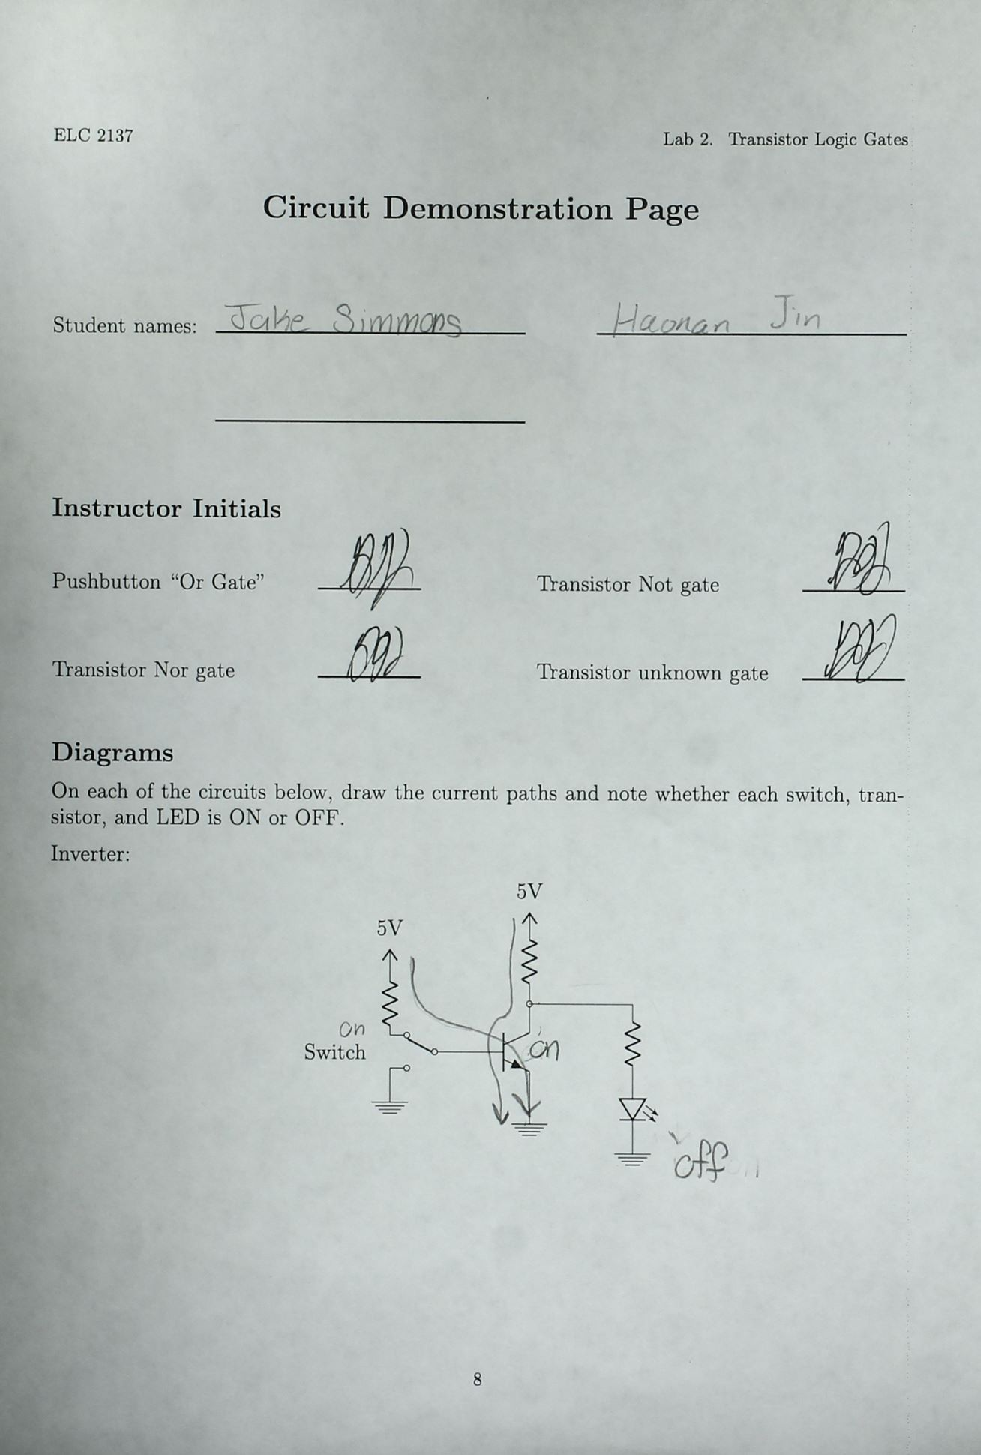
\includegraphics[width=1\textwidth,page=1]{Lab_2_Scan.pdf}
\end{figure}

\begin{figure}
		\includegraphics[width=1\textwidth,page=2]{Lab_2_Scan.pdf}
			\caption{Schematics and drawing of current path for each logic gate}
\end{figure}
\end{center}

\begin{center}
 	\caption{Table 1: Truth Table of the Final gate.}
	
	\begin{tabular}{cc|c} 
		\toprule
	 A & B & Led \\
	\midrule
	0 & 0 & 0  \\
	0 & 1 & 0 \\
	1 & 0 & 0  \\
	1 & 1 & 1  \\
	\bottomrule
	

	\end{tabular}\medskip
\end{center}


\clearpage
\section*{Code}




\end{document}
